\documentclass[a4paper,oneside,12pt]{report}
\usepackage{graphicx,mathptmx}
\usepackage{geometry}
 \geometry{
 a4paper,
 %total={160mm,227mm},
 left=40mm,
 top=25mm,
 bottom=40mm, 
 right=25mm,
}
\renewcommand{\baselinestretch}{1.5} 

\usepackage{setspace}
\usepackage{tabu}
\usepackage[acronym]{glossaries}
\makeglossaries
\usepackage{import}

\begin{document}
\begin{titlepage}
    \begin{center}
        \Large{
        \textbf{WEATHER DATA INTEGRATION AND ASSIMILATION SYSTEM}}\\
        \vspace{144pt}
  \large      
        %\vspace{1cm}
      % by
       
        
        %\vspace{1.0cm}
        
        Gihan Chanuka Karunarathne\\
        \vspace{24pt}
       % \normalsize
      178004U\\
         \vspace{72pt}
        %\normalsize
        Degree of Master of Science\\
       
        %\centering
         %\includegraphics[width=0.4\textwidth]{0.Title_Page/uom.png}\\
            %\vspace{0.8cm}
         %\normalsize
        
        %\vfill
       \vspace{72pt}
        \large
        Department of Computer Science and Engineering\\
        \vspace{24pt}
        University of Moratuwa\\
        Sri Lanka\\
        \vspace{32pt}
        April 2019
        
    \end{center}
\end{titlepage}

\begin{titlepage}
    \begin{center}
       % \vspace*{1cm}
        \Large{
        \textbf{WEATHER DATA INTEGRATION AND ASSIMILATION SYSTEM}}\\
        \vspace{144pt}
  \large      

        Herath Mudiyanselage Gihan Chanuka Karunarathne\\
        \vspace{24pt}
       % \normalsize
        178008U\\
         \vspace{72pt}
        \normalsize
        Thesis submitted in partial fulfillment of the requirements for the degree Master of Science in Computer Science and Engineering\\
     
        %\vfill
       \vspace{72pt}
        \large
        Department of Computer Science and Engineering\\
        \vspace{24pt}
        University of Moratuwa\\
        Sri Lanka\\
        \vspace{32pt}
        April 2019
        
    \end{center}
\end{titlepage}

\pagenumbering{roman}

\newgeometry{left=4cm,top=0.5cm,right=2.5cm}
\chapter*{Declaration}
\addcontentsline{toc}{chapter}{Declaration}

I declare that this is my own work and this thesis does not
incorporate without acknowledgement any material previously submitted for a
Degree or Diploma in any other University or institute of higher learning and to
the best of my knowledge and belief it does not contain any material previously
published or written by another person except where the acknowledgement is
made in the text.

Also, I hereby grant to University of Moratuwa the non-exclusive right to
reproduce and distribute my thesis/dissertation, in whole or in part in print,
electronic or other medium. I retain the right to use this content in whole or part
in future works (such as articles or books).

\vspace{0.5in}
\noindent
\begin{tabu} to 1.0\textwidth { X[l] X[l] }
    Signature: & Date:
\end{tabu}



\vspace{0.5in}
\noindent
The above candidate has carried out research for the Masters thesis under our supervision.


\vspace{0.5in}
\noindent
\begin{tabu} to 1.0\textwidth { X[l] X[l] }
    Name of the supervisor: & Dr. HMN Dilum Bandara\\ [1.5ex]
    Signature of the supervisor: & Date:
\end{tabu}

\restoregeometry
\normalsize


\newgeometry{left=2.5cm,top=0.2cm,right=2cm}
\addcontentsline{toc}{chapter}{Abstract} 
{\setstretch{1.0} 
\chapter*{Abstract}
%\chapter*{\hspace{1cm} Abstract}

To enhance the accuracy of weather predictions, it is necessary to provide reliable and detailed weather data as inputs to \acrfull{nwm}. These \acrshort{nwm} utilize weather data collected via diverse sources such as automated weather stations, radars, air balloons, and satellite images. Prior to feeding such diverse data (collected from different sources that belongs to different stakeholders) into respective \acrshort{nwm}, it is necessary to integrate data into a common format. Moreover, the data integration system’s response time need to be relatively low to accommodate critical situations like hurricanes, storms, and floods which require rapid and frequent execution of \acrshort{nwm}.

Providing public to access weather data is also useful to enable many third-party applications and research. For example, logistic companies can use those data with their own model to plan and schedule their deliveries. Agricultural insurance companies can warn the farmers in advance, as well as calculate premiums based on anticipated weather patterns.

While \acrfull{dias} and \acrfull{madis} are some of well-known Weather Data Integration and Assimilation (WDIA) systems, they are proprietary. Further Delft-FEWS is free to use, it is not open source. Hence, users of WDIA are forced to pay heavy licenses and are unable to extend the solutions to cater to their country-specific requirements. Therefore, the objective of this research is to develop a WDIA system for Sri Lanka, as well as make it open source, so that others could user and contribute to the solution.

\vspace{4mm}

\textbf{Keywords:} WDIAS, Weather, Timeseries, Distributed, Scalable

}
\restoregeometry
\normalsize

\addcontentsline{toc}{chapter}{Dedication} 
\chapter*{Dedication}
I dedicate my thesis work to my family, teachers and specially friends at \acrfull{curw}. A special feeling of gratitude to my loving parents, Nandawathi Dissanayake and H.M.K. Karunarathne whose words of encouragement and push for tenacity ring in my ears. My wife Jayani Kumarasinghe have never left my side and are very special.

I also dedicate this thesis to my many friends at \acrshort{curw} who have supported and be with me during this period of time. Also special thanks to Dr. Dilum Bandara and Dr. Srikantha Herath for giving me this wonderful opportunity to explore this new domain.

\addcontentsline{toc}{chapter}{Acknowledgements} 
\chapter*{Acknowledgements}
I wish to thank my evaluation panel members who were more than generous with their expertise and precious time. A special thanks to Dr. Dilum Bandara, my research supervisor for his countless hours of reflecting, reading, encouraging, and most of all patience throughout the entire process. Thank you Dr. Dilika Peris, and Dr. Indika Perera for agreeing to serve on my evaluation panel and Dr. Srikantha Herath for agreeing to serve as my external supervisor.

I would like to acknowledge and thank Department of Computer Science and Engineering, University of Moratuwa, for allowing me to conduct my research and providing any assistance requested. Special thanks goes to both academic and non-academic staff of the department for their continued support. I also gratitude to the University of Moratuwa for the financial support as the research was supported in part by the Senate Research Grant of the University of Moratuwa under award number SRC/LT/2017/01.

Finally, I would like to thank the teachers, evaluating panel and colleagues that assisted me with this project. Their excitement and willingness to provide feedback made the completion of this research an enjoyable experience.

\tableofcontents

\addcontentsline{toc}{chapter}{List of Figures} 
\listoffigures

\addcontentsline{toc}{chapter}{List of Tables} 
\listoftables

\addcontentsline{toc}{chapter}{List of Abbreviations} 
\printglossary[type=\acronymtype, title=List of Abbreviations, toctitle=List of Abbreviations, nonumberlist]

\pagenumbering{arabic}

\chapter{Introduction}
\label{ch:intro}
To enhance the accuracy of weather predictions, it is necessary to provide reliable and detailed weather data as inputs to \acrfull{nwm}. These NWMs utilize weather data collected via diverse sources such as automated weather stations, radars, air balloons, and satellite images. Prior to feeding such diverse data (collected from different sources that belongs to different stakeholders) into respective NWMs, it is necessary to integrate data into a common format. Moreover, the data integration system’s response time need to be relatively low to accommodate critical situations like hurricanes, storms, and floods which require rapid and frequent execution of NWMs.

\section{Motivation}
Providing public to access weather data is also useful to enable many third-party applications and research. For example, logistic companies can use those data with their own model to plan and schedule their deliveries. Agricultural insurance companies can warn the farmers in advance, as well as calculate premiums based on anticipated weather patterns.

While Data Integration and Analysis System (DIAS) and Meteorological Assimilation Data Ingest System (MADIS) are some of well-known Weather Data Integration and Assimilation (WDIA) systems, they are proprietary. Further Delft-FEWS is free to use, it is not open source. Hence, users of WDIA are forced to pay heavy licenses and are unable to extend the solutions to cater to their country-specific requirements. Therefore, the objective of this research is to develop a WDIA system for Sri Lanka, as well as make it open source, so that others could user and contribute to the solution.


\section{Problem}
\begin{itemize}
    \item Handling spatio-temporal weather data is challenging
    \item Need an extendable system to support weather models by efficiently storing and retrieving data
    \item Goal is to design and develop a Weather Data Integration and Assimilation System that,
    \begin{itemize}
        \item Integrates weather data from different sources with quality control
        \item Efficiently store spatio-temporal weather data with multiple dimensions
        \item Support geographical and time-base queries
    \end{itemize}
\end{itemize}

\section{Objectives}
\begin{itemize}
    \item To develop an open platform to integrate weather data from different sources in different formats
    \item To design and develop a schema to store multidimensional weather timeseries data while optimizing,
    \begin{itemize}
        \item Disk space
        \item Availability
        \item Access time
    \end{itemize}
    \item To optimize schema to support data queries based on geography and time
    \item To develop an API to share data while providing role-based access control
\end{itemize}

\section{Outline}
The rest of the thesis is organized as follows. Literature review is presented in Chapter \ref{ch:literature}. Solution approach with the proposed system architectures and adaptation with problem occurred are presented in Chapter \ref{ch:method}. Performance analysis is presented in Chapter \ref{ch:results} while summary and future work are presented in Chapter \ref{ch:conc}.

\chapter{Literature Review}
\label{ch:literature}
There are many of Weather forecasting, assimilation and dissemination systems developed by some of developed countries around the world as a result of trying to reduce the damage causing by natural disasters such as flood, storms, hurricanes and even for drought. Above kind of natural disasters heavily affected on the economy and the life conditions of the country, researchers have developed systems and many of these systems are using as proprietary systems. Other countries also using those systems and adopt with own version of system which effective for the specific weather condition in a particular country.
Though out this chapter includes a Literature review about existing systems and their architecture approach and design with available resources. Most influenced systems for \acrshort{wdias} is \acrshort{fews} and \acrfull{lead} system. \acrshort{fews} is an open data handling platform, but it distributed as Closed Source software. \acrshort{lead} is following the Service Oriented Architecture for system architecture. Under each system we explore both system architecture, scalability and flexibility of the system.

\section{The Delft-FEWS flow forecasting system}
 \acrshort{fews} is developed by Deltares in the Nethaland with targeted for use by operational forecasting agencies. The software is freely available to download and setup. Tutorials and User setup guide \cite{DeltaresPublicWikiDelft-FEWSGuide} are available with well documentations. For non-commercial users need to have the licence agreement to use the system. And get new system updates. However, investments in new developments in the system are normally paid for by its users. The code base of \acrshort{fews} is currently not fully open source. But configuration guides and generic adapter module integration code examples are available for the users.

Most if the models are using model-centric approach such as inputs need to be in the format of specific to the model. Also the outputs produced by the model are specific to the model and hard to utilize by another systems (e.g.,FLO2D). For the \acrshort{fews} is using much more modular approach, hence it is easy to integrate models into the \acrshort{fews} system. Thus \acrshort{fews} can be consider as an integration framework or a middle ware for the models.

Forecasting processes are constructed as a combination of modelling steps and data transformation algorithms. These are then combined to provide required forecast capabilities. Flexibility is achieved through integrating new models and algorithms into the code base \cite{Werner2013TheSystem}. Delft-FEWS system contains no inherent hydrological modelling capabilities within its code base. Rather it is a framework which can use to integrate into the system and create work flows for forecasting.

The key elements of a forecasting system are summarized by Haggett \cite{Haggett1998AnWales} as four main steps;
\begin{enumerate}
\item Detection
\item Forecasting
\item Dissemination and Warning
\item Response
\end{enumerate}
Within these four steps, \acrshort{fews} focuses on the forecasting step. The primary objective of this step is to provide additional lead time through predictions of short term future hydro-meteorological conditions \cite{Werner2005FloodCatchments}. It is true that, with providing accurate predictions with greater lead time can reduce the level of destruction. In order to do the forecasting, the system should be capable of integrating real-time data from hydrological and meteorological observation networks, and the dissemination of prediction results through appropriate products to the warning process.

In figure \ref{fi:fews_schematic} show a schematic view of the connection between the forecasting system to real time data acquisition systems and dissemination systems. The widely using concept is using meteorological forecast data to get precipitation and, then using hydrological and hydraulic model chain to predict the level affect on the ground. The hydrological and hydraulic model should be design based on the ground. Basically ground should be analyze geographically and divide into the catchments. Based on the affected catchment, it can be further divide into sub areas in order to reduce the complexity of the simulation task. Ideally the forecasting system should therefore be flexible to allow change to models and data, while keeping the way forecasters work with it as constant as possible.
 
\begin{figure}[htp]
    \centering
    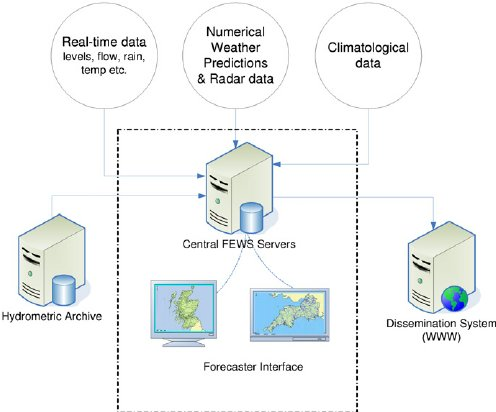
\includegraphics[width=0.7\textwidth]{images/fews/Schematic-structure-of-a-fl-ood-forecasting-system-showing-the-position-of-Delft-FEWS_W640.jpg}\\
    \caption{Schematic structure of a flood forecasting system, showing the position of \acrshort{fews} and links to other primary systems within the operational environment. \cite{Werner2013TheSystem} }
    \label{fi:fews_schematic}
\end{figure}
The foundation of \acrshort{fews} is data-centric, with a common data-model through which all components interact. All time series data (both scalar and gridded) are stored in this common data-model in a database. Modeling capabilities are then linked to the system through one of the interfaces provided to the data-model \cite{Werner2013TheSystem}. As mention in the paper, having a common data-model make easy to store data in an efficient way. Operations like reporting and sharing the data also make it easy for integrate models. But the problem with this approach is, handling the multiple data formats. \acrshort{fews} overcome this issue with introducing adapters for most of commonly used data formats. This is a good feature which enable users to easily import data into the system. But at the same time, it's adding additional complexity into the system.

Time series data is additionally either scalar, vector, or gridded data, though all different types are uniformly stored as binary objects in a time series table. None of the functional components (including the linked models) have direct access to the times series table, which is accessible only through the data access module \cite{Werner2013TheSystem}. As it explained in the system interpretation, every time all the data access need to go through the data access module which causing to adding more cost in data access. Since it is storing the different data types as binary objects, there is a penalty in converting data into binary objects and vice a versa. Storing all the data in a time series table causing all the request come into a single data point. Even it gives the advantage of accessing all the data at one place. Since screaming big amount of data is causing a heavy load on the system, causing to slow down the performance on trying to use the system on large set of data.

Given above drawback on storing the data in the system, within the \acrshort{fews} data model, time series are uniquely identified by their location and data type, as well as an id related to the source of the data (e.g.,the external source or hydrological model of which the time series are a result) \cite{Werner2013TheSystem}. This gives an opportunity to index the data base on above key fields and store the data separately, in order to take the advantage of putting multiple data resources into the system. As an example, instead of storing the data at a single timeseries table, it is possible to separate and index the database based on source such as external source or hydrological model of which the time series are a result. Or separate by data type and store in multiple storage give the capability for the system to scale with factor of identical types that can be identified. Example of separation by data types of scalar, vector and gridded will increase the scaling factor by 3x.

Data processing and manipulation is a required process in weather forecasting. Most of the data that is imported from external sources is not at the appropriate temporal and spatial scale to be applied as an input to a forecasting model, or to be used directly in product generation. As a consequence, generic data processing steps form the predominant effort in most applications of models in the forecast environment. Some examples include data validation, serial and spatial interpolation, aggregation and dis-aggregation, and merging data \cite{Werner2013TheSystem}. This a vital feature in a forecasting system, and affect on the quality and accuracy of the predicted data outputs. Because of the common data model concept in the \acrshort{fews}, data processing via these function is much effective. The system is self provided some of the generic functions for data processing, but for more complex algorithms can be developed as a new Java class coded to communicate with the application programming interface (API). It obvious that for additional feature integration, user should implement the new functional extensions via Java programming language. Users does not have the flexibility of develop with some other languages they are familiar with or use the support from another language. As an example, Python language is easy to use for beginners and many of data scientists are using this programming language for development and it has many data available libraries for data processing. But in the \acrshort{fews} users do not ave the capability to take the advantage of such existing things.

\begin{figure}[htp]
    \centering
    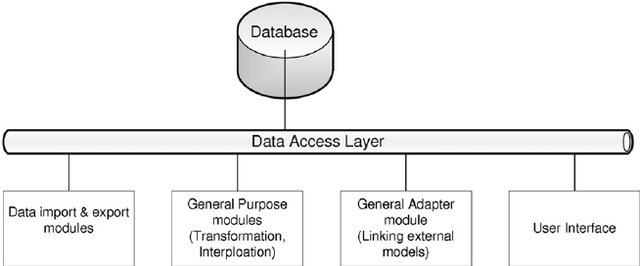
\includegraphics[width=1.0\textwidth]{images/fews/Architecture-of-Delft-FEWS-showing-the-data-base-the-data-access-layers-and-examples-of_W640.jpg}\\
    \caption{Architecture of \acrshort{fews} showing the data base, the data access layers and examples of functional modules that communicate through the data access layer. \cite{Werner2013TheSystem} }
    \label{fi:fews_data_layer}
\end{figure}
Most of the library of functions provided work equally on scalar and gridded time series. As with all other modules this communicates with the database solely through the data access layer as shown in \ref{fi:fews_data_layer} \cite{Werner2013TheSystem}. As it shown in the figure, it is clearly showing that, the system is depends on single database and via the data access layer all the requests are coming to the database though a connection. It is possible to setup and connect to a enterprise level database with clustering and shading as a paid solution, in order to serve many requests as possible. But the design it self inherently suffer with the database bottleneck which effected on running a large set of timeseries or models.

\begin{figure}[htp]
    \centering
    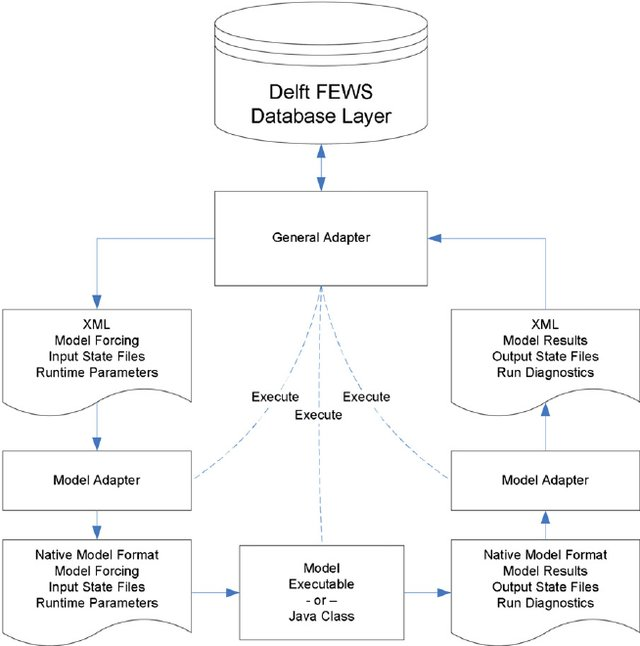
\includegraphics[width=0.8\textwidth]{images/fews/Linking-Delft-FEWS-with-external-models-The-fi-gure-shows-the-fl-ow-of-data-through-XML_W640.jpg}\\
    \caption{ Linking \acrshort{fews} with external models. The figure shows the flow of data through XML and native model formats using solid lines, while executable commands are shown by dashed lines. \cite{Werner2013TheSystem} }
    \label{fi:fews_general_adapter}
\end{figure}
On of the simple and most effective feature in the \acrshort{fews} is open approach to integration of models and data. This approaches the concept of the open modeling framework proposed by \cite{Kokkonen2003InterfacingXML}. It simply gives the flexibility to allow operators to integrate more models as well as variations of the same model and come up with new integration flows as much as possible.
\acrshort{fews} generates the input data as a set of XML files to a defined location; an adapter developed specifically for the model in question transforms this to the required native format in a pre-processing step; \acrshort{fews} executes the model; and the adapter to that model then converts the native formatted results into XML formatted files in a post processing step. \acrshort{fews} subsequently imports the results into the database from the XML files (see Fig. \ref{fi:fews_general_adapter}) \cite{Werner2013TheSystem}. The process is simple and consistence through out all the model integration. The model execution is done by the \acrshort{fews} or the model adapter which is causing tide coupling into the execution process in the system. Users does not have the flexibility to run the models with different configurations such as running with parallel execution. That may be overcome by triggering a external process at the execution time, but it introducing more difficulty for handling after model executed successfully, preceding to the next step in the process. This part of the system feature is not focus on the \acrshort{wdias} and user has to come up with own flow or use existing scientific flow management system. But it is a concept that need to be discuss and understand properly in order to design a data integration and assimilation system.

Exchanging data with the model is primarily through XML files. In some cases these XML files may become very large, which may lead to I/O bottlenecks and subsequent performance issues \cite{Werner2013TheSystem}. This issue is thoroughly discussed previous paragraphs and the authors of the \cite{Werner2013TheSystem} seems to be notice and accept it here. For overcome this issue they introduced the file-based exchange of data. This includes the use of binary-XML files, streaming files through memory, and the use of \acrshort{NetCDF}-CF files. But far as for users it seems to be adding more complexity and context in order to get higher performance via the system.

If particular adapter for a model is not present in the list of \acrshort{fews} adapter, user has the flexibility to implement an adapter for it. The effort of developing an adapter for a model code not previously integrated with \acrshort{fews} will vary depending on the complexity of the model I/O formats \cite{Werner2013TheSystem}. If user wants to use existing adapter and need to configure something not supported via the existing adapter, it is hard to get done. Also there are some cases it is hard to develop an adapter or running alongside with the \acrshort{fews}. As an example FLO2D model is using for hydrologic modeling and the model is only support only on Windows based operating systems. If you setup the system on Linux base operating system and using Linux based models, it is hard for users to come up with a solution for integrating the FLO2D models.
The final step and one of important feature is exporting the data from the system in useful manner. In the \acrshort{fews}, it is supporting three main forms of product generation.
\begin{itemize}
\item Generate web reports with graphs, tables as well as summary reports
\item Export time series in a variety of formats
\item External applications actively retrieve data from the system
\end{itemize}
The forecasting process is often a sequence of steps, starting with the import of data, a number of data processing and modeling steps, and culminating in the generation of products to be disseminated to the warning process. This is supported via the work flow process in the \acrshort{fews}. The scope of the \acrshort{wdias} is not focus on adding such a feature in the system, rather user have to use scientific work flow management system or come up with own version of work flow.

When running sequential steps within a work flow in \acrshort{fews}, each step is run for the full time window required (e.g.,the lead time of the forecast) before moving on to the next step. This precludes tightly coupling of models, even explicitly \cite{Werner2013TheSystem}. As it mentioned above, users can run multiple models parallel or run those sequentially as needed. 

\section{Linked Environments for Atmospheric Discovery}

The reason behind developing \acrfull{lead} by US National Science Foundation (NSF)  is to addresses the fundamental research challenges needed to create an integrated, scalable framework for adaptive analyzing and predicting the atmosphere \cite{Droegemeier2005Service-OrientedWeather}. In order to predict and analysis weather models by researchers, it required many resources. Rather than each researcher is running and handling own computer resources to do the weather experiments, \acrshort{lead} is providing pool of resources, then the researchers can use this resource pool to run their experiment in shorter amounts of time and in higher scale. At the time, researchers are developing their experiment flow, they are not using the resources many, and other are using it at the same time. LEAD’s foundation is dynamic work flow orchestration and data management in a Web services framework \cite{Droegemeier2005Service-OrientedWeather}.

The most relevant and important analysis for designing \acrshort{lead} is understanding and analyzing the \acrfull{lead} architecture of it. LEAD’s complex array of services, applications, interfaces, and local and remote computing, networking, and storage resources is assembled by users in work flows to study mesoscale weather as it evolves \cite{Droegemeier2005Service-OrientedWeather}. As it follows the \acrshort{soa}, everything is implemented as independent services. This enable \acrshort{lead} to scale each service as required, and update each service without affecting other services. New models which are required for implementing a new forecast flow also has to be implement as a service and then integrate into the system.

In the \ref{fi:lead_system} shows the fundamental capabilities of the \acrshort{lead} system. 
From the high-level view, \acrshort{lead} lets users query for and acquire information, simulate and predict weather by using numerical atmospheric models, assimilate data, analyze, mine, and visualize data and model output.

\begin{figure}[htp]
    \centering
    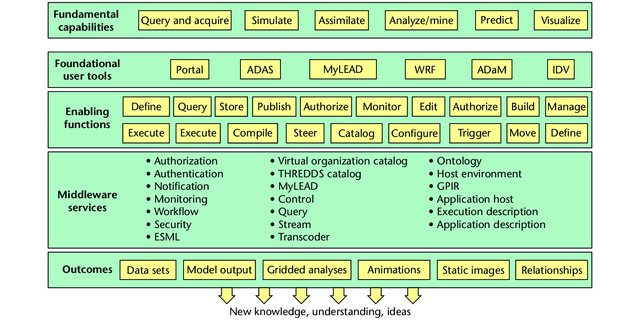
\includegraphics[width=1.0\textwidth]{images/lead/LEAD-system-Fundamental-capabilities-familiar-to-meteorologists-are-shown-in-the-top_W640.jpg}\\
    \caption{LEAD system. Fundamental capabilities familiar to meteorologists are shown in the top level, below which are the associated tools for enacting these capabilities and the middle-ware that links everything together. System-generated products appear at the bottom. \cite{Droegemeier2005Service-OrientedWeather} }
    \label{fi:lead_system}
\end{figure}

The second level in \ref{fi:lead_system} contains the fundamental tools that help to link services together. This include following tools in brief \cite{Droegemeier2005Service-OrientedWeather};
\begin{itemize}
    \item a Web portal, the primary (though not exclusive) user entry point
    \item the ARPS Data Assimilation System (ADAS), a sophisticated tool for data quality control and assimilation
    \item myLEAD, a flexible metadata catalog service
    \item \acrfull{wrf} a next-generation atmospheric prediction and simulation model
    \item ADaM (Algorithm Development and Mining), a powerful suite of tools for mining observational data, assimilated data sets, and model output 
    \item Integrated Data Viewer (IDV) 
\end{itemize}

\begin{figure}[htp]
    \centering
    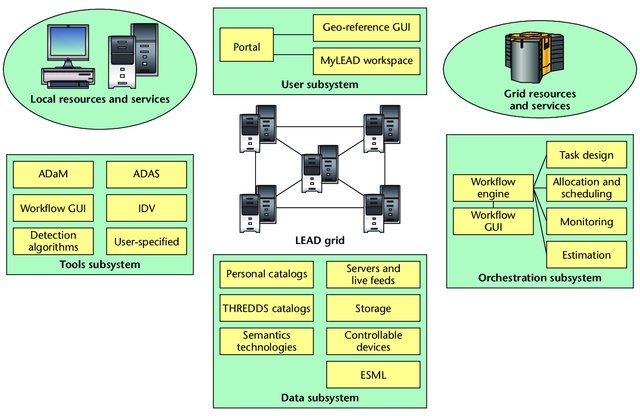
\includegraphics[width=1.0\textwidth]{images/lead/LEAD-system-framework-LEAD-is-composed-of-several-interacting-subsystems-with-the-LEAD_W640.jpg}\\
    \caption{ LEAD system framework. LEAD is composed of several interacting subsystems, with the LEAD grid representing a stable, secure environment for development and testing. \cite{Droegemeier2005Service-OrientedWeather} }
    \label{fi:lead_framework}
\end{figure}

The Concept of the \acrshort{lead} is, the workflow orchestration for on-demand, real-time, dynamically adaptive systems, called as WOORDS. The system is doing the work flow orchestration as given in each procedure. Those procedural rules are define by researcher and feed into the system. The system is trying to perform the action immediate after the submission, and also it transmit the data, run the models and send back the put put with lower time delay as possible. According to the load and other requirement, the system will respond to those requirements automatically.

Lead System is consist of following sub components, as shown in the \ref{fi:lead_soa}. As a brief summary of the subsystems is \cite{Droegemeier2005Service-OrientedWeather};
\begin{itemize}
\item User subsystem - comprises the LEAD portal and enable user can access services
\item Data subsystem - handles data and metadata, any numerical model output produced by operational or experimental models, and user generated information.
\item Tools subsystem - consists of all meteorological and IT tools
\item Orchestration subsystem - provides the technologies that let users manage data flows and model execution streams, and create and mine output. It also provides linkages to other software and processes for continuous or on-demand applications. 
\end{itemize}

\begin{figure}[htp]
    \centering
    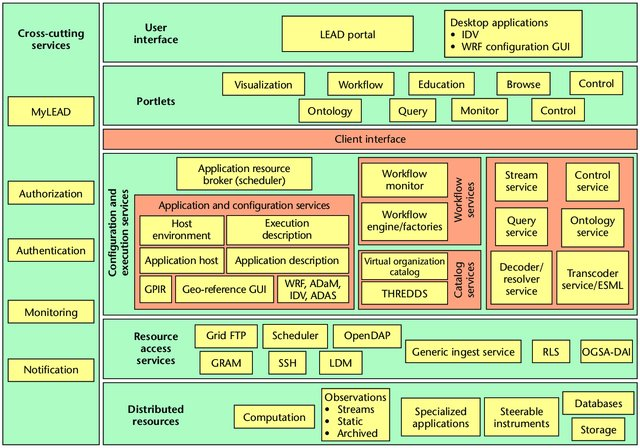
\includegraphics[width=0.9\textwidth]{images/lead/LEADs-service-oriented-architecture-A-wide-variety-of-services-and-resources-grouped_W640.jpg}\\
    \caption{LEAD’s service-oriented architecture. A wide variety of services and resources, grouped here according to general functionality, comprise the LEAD architecture, including services that cut across all aspects of the system. \cite{Droegemeier2005Service-OrientedWeather} }
    \label{fi:lead_soa}
\end{figure}

The distributed computing systems in the LEAD grid represent a distributed test bed for developing, integrating, and testing LEAD’s components.

\acrshort{soa}s are widely deployed in the commercial enterprise sector, and they form the foundation of many scientific “grid” technologies at the time of \acrshort{lead} design and developed. A variant of \acrshort{soa} is evolved later called as microservice architecture, and widely use in the industry nowadays. The \acrshort{lead} \acrshort{soa} has five distinct yet highly interconnected layers. 

The bottom layer represents raw computation, application, and data resources distributed throughout the LEAD grid and elsewhere. The next level up holds the Web services that provide access to raw services \cite{Droegemeier2005Service-OrientedWeather}. These two layers are working together, since \acrshort{lead} system resources are distributed over multiple locations and creating a pool of resources. The upper layer to the raw resources is abstracting the complexity of managing and accessing the resources, and provide a simplified access to the upper layer. In the Upper layers, it view as a unlimited resource pool for storing and handling data.

The configuration and execution services in the middle layer, consisting of five elements, represent services invoked by LEAD workflows. These are some critical aspects on a weather data management system. Most of the services listed here are required for creating work flows for weather data forecasting. Thus it is important to review them and understand the basic needs of a weather data management system.

\begin{itemize}
\item The application-oriented configuration service that manages the deployment and execution of real applications such as the \acrshort{wrf} simulation model, ADAS, and the ADaM tools \cite{Droegemeier2005Service-OrientedWeather}. When creating weather work flow, it is required to change the behaviour of model by changing some of the configurations of the model or run a different version of the model.
\item The application resource broker, which matches the appropriate host for execution to each application task, based on the execution’s time constraints \cite{}. This service is a critical part of the system, and responsible of using the resources of the system in optimized manner. When designing the weather data system, it is required to increase the capacity of the system automatically, and adopt into the system.
\item The workflow engine service, which drives experimental workflow instances, invokes both the configuration service and application resource broker \cite{Droegemeier2005Service-OrientedWeather}. This is a part of work flow orchestration.
\item The catalog services, represents the manner in which a user or application service discovers public-domain data products, or \acrshort{lead} services \cite{Droegemeier2005Service-OrientedWeather}. This is an important feature that should be available in a weather data system, and it is important to users to search for the availability of the data. Further wants to analyze the existing data for decision making.
\item Users require a host of data services to support rich query, access, and transformation operations on data products. An important goal behind LEAD is access transparency—facilitating user queries across all available heterogeneous data sources without adverse affects from different formats and naming schemes \cite{Droegemeier2005Service-OrientedWeather}. Users need to have transformation services to read data in different format. The query service gives the capability to search via available data without any affect on the data formats.
\end{itemize}
The top of the \ref{fi:lead_soa}, shows the user interface to the system. This give the access to individual services. When user logs into the system, based on the authentication and authorization setting bind to the individual account, the portlets can access the services on behalf of the user. Look into further details is not relevant to developing the \acrshort{wdias}, since the focus is not about workflow orchestration.

\acrshort{lead} is a more advanced system which can support for mesoscale weather prediction with the effort of multiple universities in the United State America with the effort of many of researchers and using many of computer resources. At the time it was building, it uses the \acrshort{soa} architecture as into its depth, and with the implementation each service can scale as needed and possible to enhance the service without interrupting other services. In the \acrshort{wdias} only focus on creating a framework that is extendable as system need more features as like \acrshort{lead} services.

\section{Data Integration and Assimilation System}
\label{se:dias}

\section{Meteorological Assimilation Data Ingest System}
\label{se:madis}

\section{Summary}


\chapter{Method}
\label{ch:method}


Reviews literature and place your work within the existing body of literature here. In chapter \ref{ch:intro} you introduced your thesis.

\section{Introduction}

\section{Service Oriented Architecture}

\section{Microservice Architecture}

\section{Hierarchical Database Structure}

\section{Weather Data Prepossessing}

\subsection{Interpolation}

\subsection{Transformation}

\subsection{Validation}

\section{Query Timeseries}

\chapter{Results}
\label{ch:results}

\section{Test Plan}

\section{Work Load Creation}

\section{Observations}

\chapter{Conclusions}
\label{ch:conc}

Discuss your results and system and conclude.

\section{Summary}

\section{Future Work}

\appendix
\chapter{First Appendix}
Type out your first appendix here.
\section{Basics}

\chapter{First Appendix}
Type out your second appendix here.

\graphicspath{ {./images/} }
\newacronym{wdias}{WDIAS}{Weather Data Integration and Assimilation System}

\newacronym{fews}{Delft-FEWS} {Delft-FEWS, Deltares}
\newacronym{lead}{LEAD}{Linked Environments for Atmospheric Discovery}
\newacronym{dias}{DIAS}{Data Integration and Assimilation System}
\newacronym{madis}{MADIS}{Meteorological Assimilation Data Ingest System}

\newacronym{nwm}{NWMs}{Numerical Weather Models}
\newacronym{NetCDF}{NetCDF}{Network Common Data Form}
\newacronym{soa}{SOA}{Service Oriented Architecture}
\newacronym{wrf}{WRf}{Weather Research and Forecast}
\newacronym{esb}{ESB}{Enterprise Service Bus}
\newacronym{microservice}{Microservice}{Microservice Architectire}

\newacronym{curw}{CUrW SL}{Urban Center for Water, Sri Lanka}
\bibliographystyle{plain}
\bibliography{mendeley}
\end{document}